\documentclass[a4paper,10pt,twoside]{article}
\usepackage[utf8]{inputenc}
\usepackage[french]{babel}
\usepackage[T1]{fontenc}
\usepackage{amsmath}
\usepackage{amsfonts}
\usepackage{amssymb}
\usepackage{graphicx}
\usepackage{multicol}
\usepackage{array}
\usepackage{float}
\usepackage{epstopdf}
\usepackage[justification=centering]{caption}
\usepackage{caption}
\usepackage{subfig}
\usepackage{gensymb}
\usepackage[bottom]{footmisc}
\usepackage{appendix}
\usepackage{pdfpages}
\usepackage{todonotes}
\usepackage{mathpazo}
\usepackage{titleps}
\usepackage{color}
\usepackage{hyperref}
\usepackage[skins]{tcolorbox}
\usepackage{sectsty} 
\usepackage[arrowmos]{circuitikz}
\usepackage{pgfplots}
\usepackage{blindtext}
\usepackage{adjustbox}
\usepackage[inner=2.5cm,outer=2.5cm,top=3cm,bottom=3cm]{geometry}


\graphicspath{{figures/}}
\setlength\parindent{0pt}
\renewcommand*\rmdefault{ppl}
\newcolumntype{C}[1]{>{\centering\let\newline\\\arraybackslash\hspace{0pt}}m{#1}}
\newcolumntype{R}[1]{>{\raggedright\arraybackslash}p{#1}}
\sectionfont{\large}
\subsectionfont{\normalsize}

% Page style definitions
\newpagestyle{main}{
	\sethead[Club ELEC : Hands-on 1][][]  % even
			{\chaptertitle}{}{Club ELEC : Hands-on 1}
	\headrule
    \setfoot[\thepage][][]
    		{}{}{\thepage}		
}

\newpagestyle{appendix}{
	\sethead[Club ELEC : Annexes][][]  % even
			{}{}{Club ELEC : Annexes}
	\headrule
    \setfoot[\thepage][][]
    		{}{}{\thepage}
    \footrule
}

%----------------------------------------------------------------------------------------
%	TITLE SECTION
%----------------------------------------------------------------------------------------
\title{	
	\vspace{2.5cm}
	\normalfont \normalsize 
	\huge Club ELEC\\ 
	\vspace{2.5cm}
	\huge Projet Robot\\
	\vspace{.25cm}
	\Large HO1 - Contrôle des moteurs
	\vspace{2.5cm}
	\centering
}

\begin{document}
\renewcommand{\figurename}{Figure}
\renewcommand{\thepage}{\roman{page}}
\setcounter{page}{1}

\pagenumbering{gobble}
\maketitle
\newpage
\pagenumbering{arabic}
\pagestyle{main}

\newpage
\null
\thispagestyle{empty}
\newpage
\clearpage

\setcounter{page}{1}

%%% Introduction
\section*{Introduction}
Pendant ce quadrimestre, le Club ELEC vous propose de développer une chaine de conditionnement pour un signal audio, provenant par exemple d'un ordinateur, smartphone, etc. Pour ce faire, le développement du circuit se déroulera en 3 phases, chacune correspondant à une séance de hands-on proposée par le club.

\begin{itemize}
	\item[-] HO1: Contrôle du volume sonore.
	\item[-] HO2: Filtrage du contenu fréquentiel.
	\item[-] HO3: Distortion du signal audio.
\end{itemize}

%%% Objectifs du HO1
\section*{Objectifs}
% Objectifs: prise en main du micro et du signal sonore, notion AC/DC, utilisation de l'oscilloscope, découplage AC

Les objectifs du premier hands-on sont:

\begin{itemize}
	\item[-] De se familiariser avec le matérial de base (breadboard, multimètre, oscilloscope) et les composants de base (résistances, capacités, amplificateurs opérationnels, composants intégrés) propres à l'électronique.
	\item[-] De comprendre le fonctionnement du micro qui assure la transduction du signal sonore en signal électrique.
	\item[-] De faire le lien entre le signal obtenu et son contenu fréquentiel afin de comprendre la notion de filtrage.
	\item[-] De comprendre la notion AC/DC et le découplage AC.
	\item[-] D'implémenter en pratique la première partie du circuit (micro, filtre et découplage).
\end{itemize}

\begin{figure}[!ht]
	\centering
	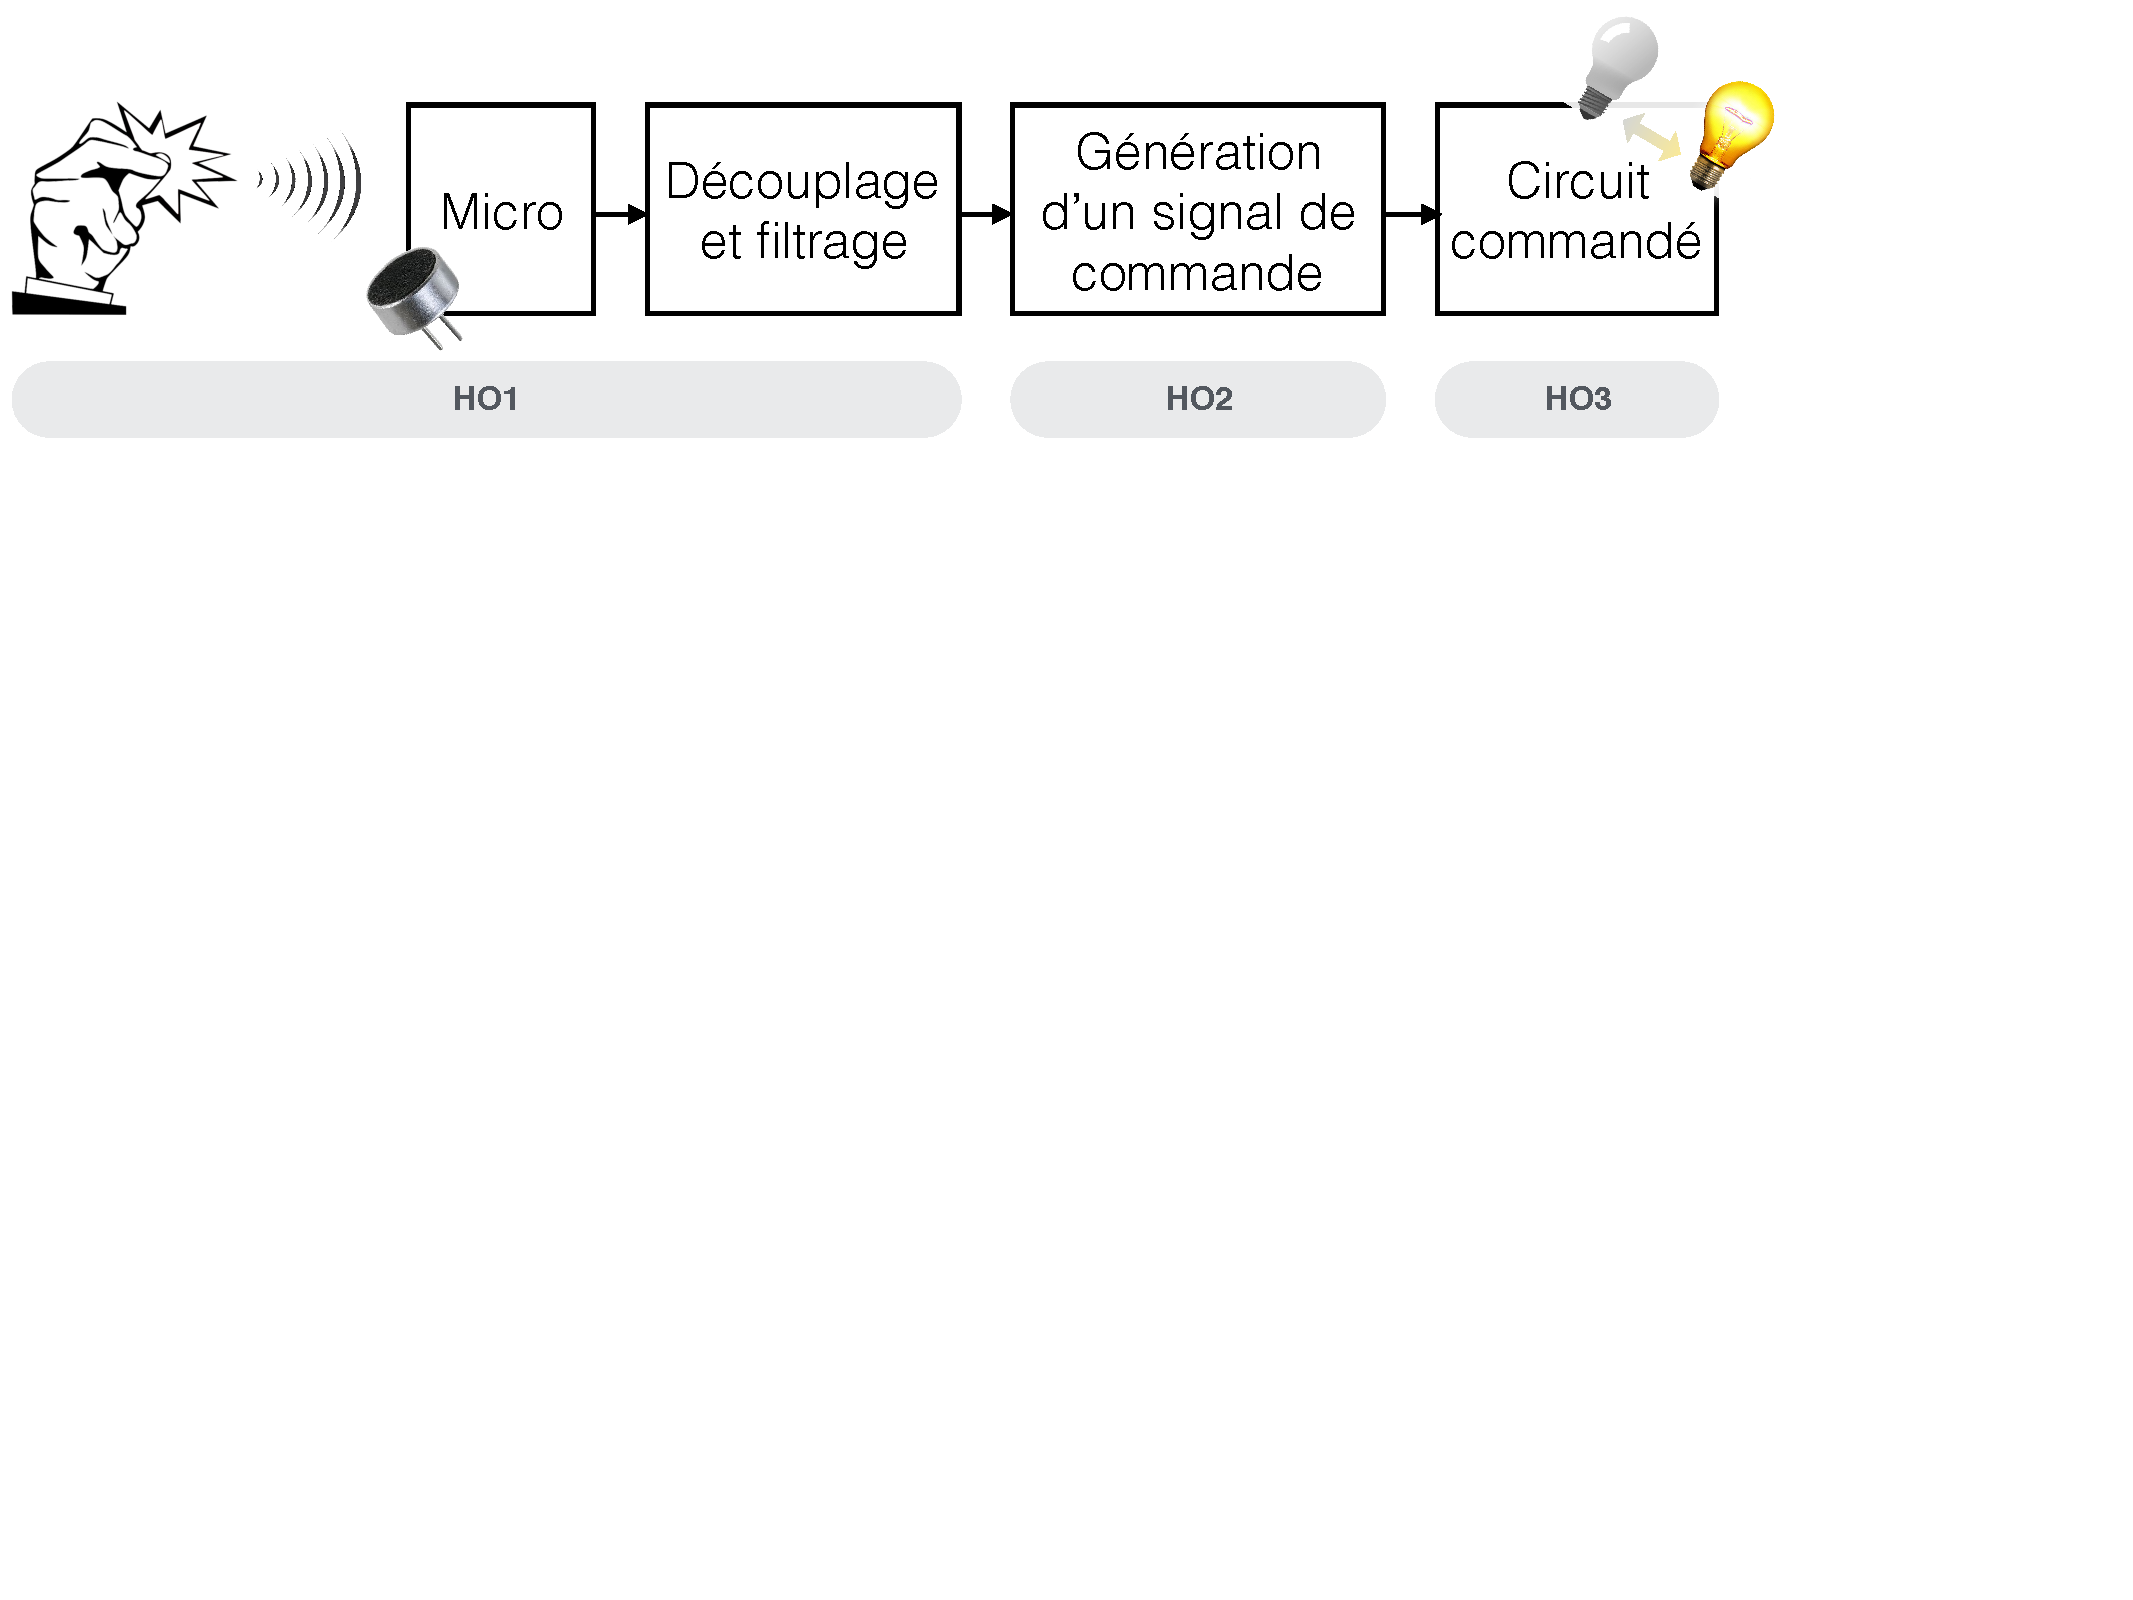
\includegraphics[width=.75\textwidth]{figures/SchemaBloc.pdf}
	\caption{Schéma-bloc du circuit.}
	\label{fig:block-diagram}
\end{figure}

Le schéma-bloc du circuit est présenté à la Figure \ref{fig:block-diagram}. Les ondes acoustiques générées par le claquement de doigt sont captées par le micro qui les transforme en un signal électrique (transduction). Ce signal est ensuite découplé et filtré à l'aide d'un filtre RC, comme présenté plus loin dans ce document. La génération d'un signal de commande propre ainsi que l'implémentation d'un circuit commandé seront abordées plus en détail dans les prochain hands-on.


%%% Description du circuit
\section*{Moteur DC}
Les moteurs utilisés pour ce projet sont des moteurs DC à balais. Ce type de moteur ne nécessite qu'une source de tension DC pour l'alimenter, au contraire de moteurs synchrones ou asynchrones, basés sur des alimentations triphasées ou N-phasées.\\

\begin{minipage}[t]{.45\textwidth}
	\centering
	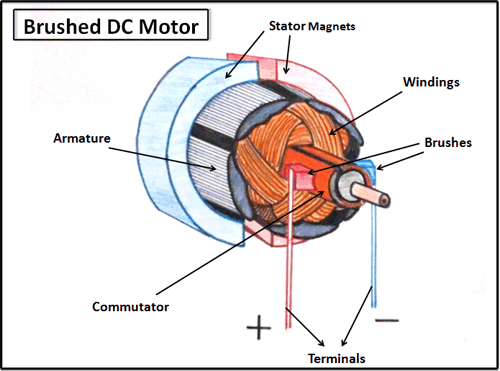
\includegraphics[width=\textwidth]{dc_motor}
	\captionof{figure}{Schéma d'un moteur DC.}
	\label{fig:dc_motor}
\end{minipage}
\hfill
\begin{minipage}[t]{.45\textwidth}
	\centering
	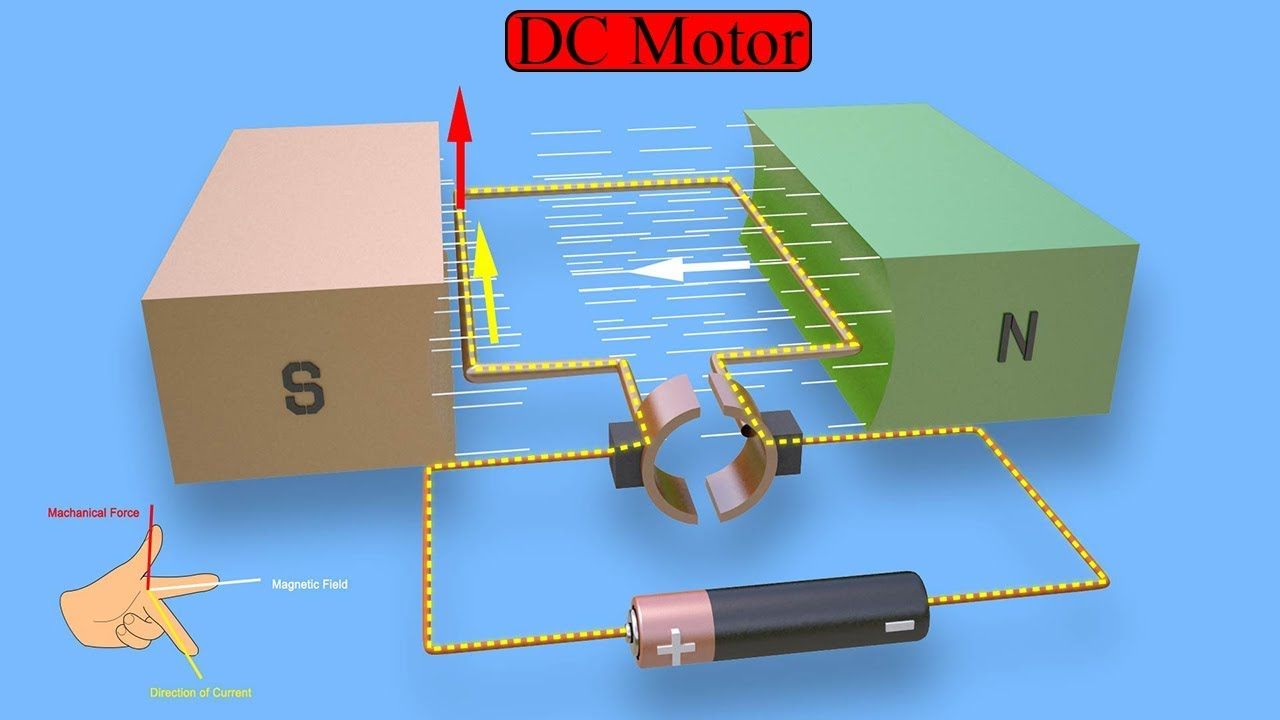
\includegraphics[width=\textwidth]{dc_motor_principle}
	\captionof{figure}{Principle de fonctionnement du moteur DC.}
	\label{fig:dc_motor_principle}
\end{minipage}
\vspace{.25cm}

Le moteur est constitué de deux pièces principales, comme illustré à la Figure \ref{fig:dc_motor}. D'une part, un \textbf{stator}, élément fixe du moteur, sur lequel on trouve généralement une structure formée d'aimants permanents, servant à générer un champ magnétique de direction fixe. D'autre part, un \textbf{rotor}, élément mobile du moteur, sur lequel on trouve généralement des bobinages alimentés par la tension DC fournie au moteur, servant à générer un champ magnétique de direction variable.\\

Le couple électro-mécanique produit par le moteur résulte du moment de force qui tend à aligner les directions des champs magnétiques générés respectivement par les aimants permanents au stator et les bobinages au rotor, comme représenté à la Figure \ref{fig:dc_motor_principle}. Un commutateur auquel les bobinages sont connectés au travers d'un système de balais, permet de choisir quels bobinages alimenter, de façon à constamment désaligner le champ magnétique résultant des bobinages par rapport à celui des aimants. C'est ce principe qui permet de produire un mouvement rotatif continu.\\

D'un point de vue purement électrique (et pour votre information uniquement, pas besoin de comprendre les détails), le fonctionnement du moteur DC est régi par 2 équations principales:

\begin{align*}
	\left \lbrace
	\begin{aligned}
		V_a &= R_a I_a + L_a \frac{dI_a}{dt} + k \phi \omega_m\\
		C_{em} &= I \frac{d\omega_m}{dt} = k \phi I_a
	\end{aligned}
	\right. 
\end{align*}

La \textbf{première équation} relie la tension d'alimentation du moteur, notée $V_a$, au courant circulant dans les bobinages, noté $I_a$ et à la force électromotric induite (le terme $k \phi \omega_m$) qui fait directement intervenir la vitesse de rotation du moteur $\omega_m$. La \textbf{seconde équation} relie le couple électro-mécanique, noté $C_{em}$ et proportionel à la dérivée de la vitesse de rotation $\frac{d\omega_m}{dt}$, au courant dans les bobinages.\\

La conclusion principale à tirer de ces équations est qu'il est possible de contrôler la vitesse du moteur $\omega_m$ uniquement en modulant la tension $V_a$ appliquée au moteur.

\section*{Pont H}
Le pont H est une structure qui permet à la fois de \textbf{déterminer le sens de rotation} du moteur, mais également de \textbf{régler la vitesse de rotation} du moteur, notée $\omega_m$ dans les équations précédentes.\\

Le pont H est basé sur 4 interrupteurs dont les connexions vont permettre de changer le sens de la tension imposée au moteur, comme illustré à la Figure \ref{fig:h_bridge_principle}. Ce changement de sens de la tension permet de faire tourner le moteur DC dans les 2 sens de rotation possibles. Il est également possible de freiner le moteur en activant les 2 interrupteurs inférieurs (ou supérieurs) pour le court-circuiter. \\

\begin{figure}[!ht]
	\centering
	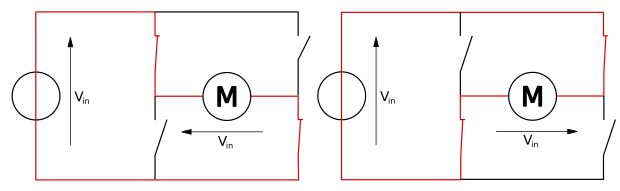
\includegraphics[width=.8\textwidth]{h_bridge_principle}
	\captionof{figure}{Principe de fonctionnement du pont H.}
	\label{fig:h_bridge_principle}
\end{figure}

Le réglage de la vitesse de rotation du moteur est réalisé par une modulation de la tension appliquée au moteur, appelée \textbf{modulation à largeur d'impulsion} (MLI). De façon générale, la source $V_{in}$ est une batterie et fournit une tension DC fixe dont il n'est pas possible de modifier la valeur, alors que cela est pourtant nécessaire pour pouvoir contrôler le moteur. La solution trouvée pour contourner ce problème consiste à moduler le rapport cyclique de la tension appliquée au moteur en connectant et déconnectant les switches du pont H. De cette façon, la valeur moyenne du signal (courbe rose sur la Figure \ref{fig:pwm_principle}) correspond à la valeur souhaitée (courbe verte sur la Figure \ref{fig:pwm_principle}). On arrive donc bien à générer une tension variable sur base d'une batterie fournissant une tension fixe.\\

En termes d'implémentation, le circuit du pont H est présenté à la Figure \ref{fig:h_bridge}. Les interrupteurs sont généralement implémentés sur base de transistors (bipolaires ou MOS) qui se trouveront ici dans le composant intégré (L293D). Les diodes mises en parallèle avec les interrupteurs sont des composants primordiaux pour assurer le bon fonctionnement du pont. En effet, le moteur étant constitué de bobinages qui présentent un comportement essentiellement inductif, le courant qui traverse ces bobinages ne pourra pas passer immédiatement à zéro lorsque l'on ouvre les interrupteurs. Les diodes sont donc là pour fournir un chemin au travers duquel peut passer ce courant, évitant ainsi d'endommager les interrupteurs.

\begin{minipage}[t]{.45\textwidth}
	\centering
	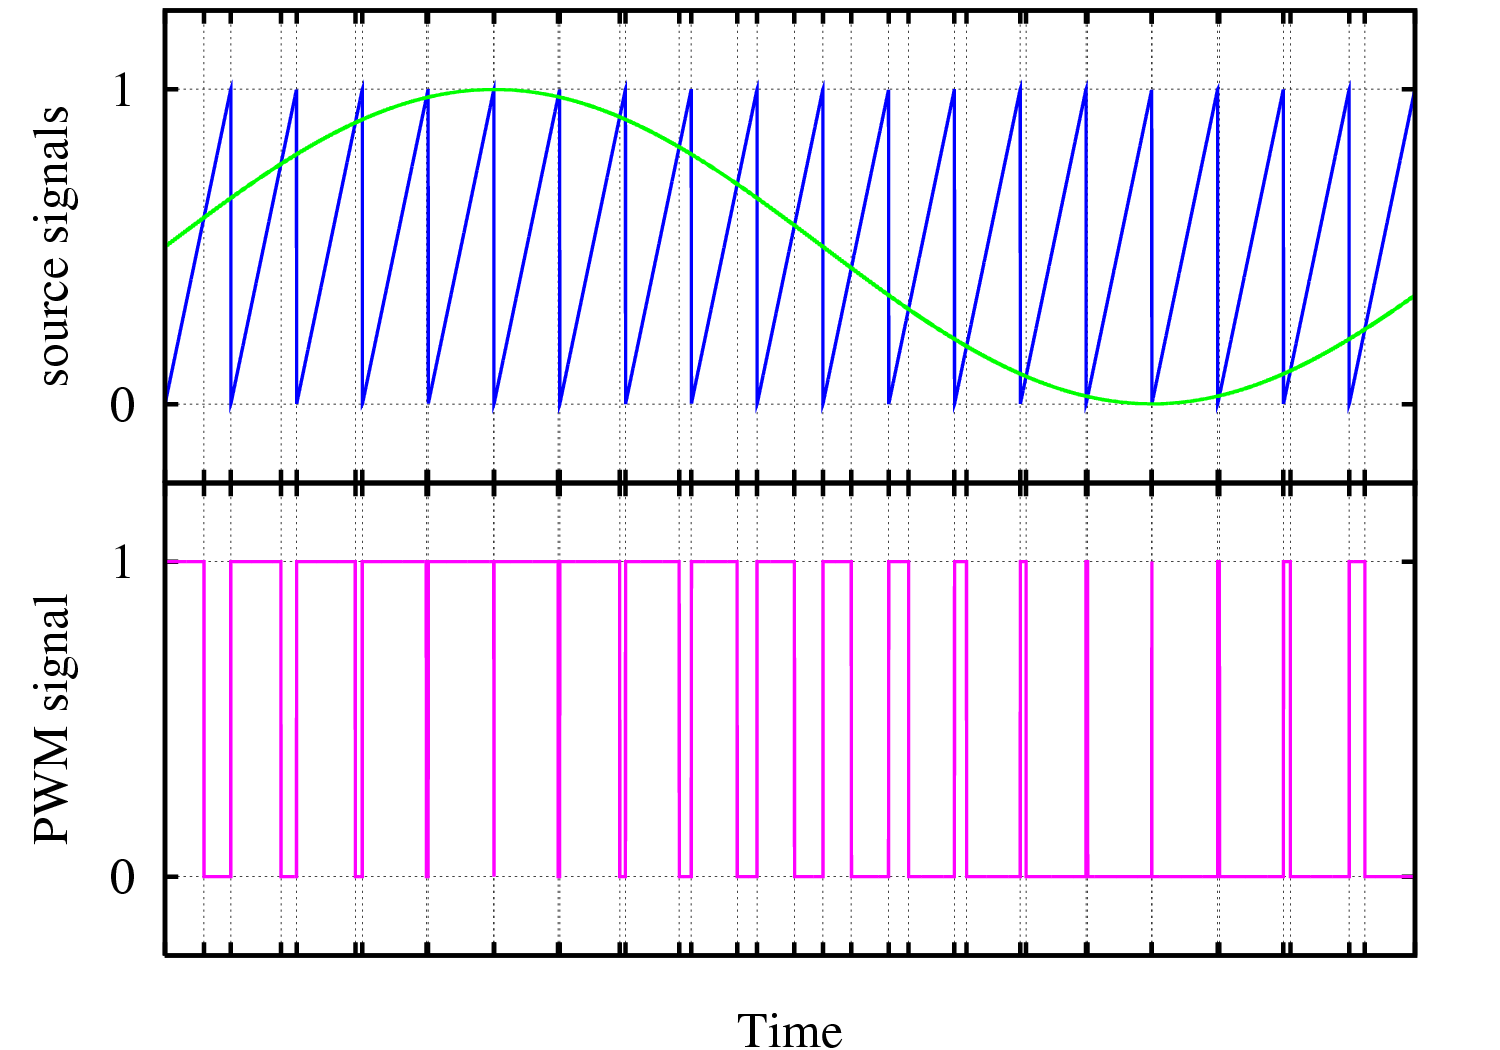
\includegraphics[width=\textwidth]{pwm_principle}
	\captionof{figure}{Modulation à largeur d'impulsion (MLI).}
	\label{fig:pwm_principle}
\end{minipage}
\hfill
\begin{minipage}[t]{.45\textwidth}
	\centering
	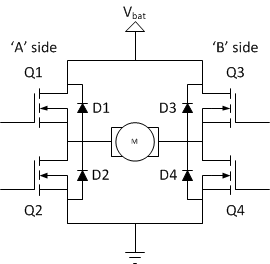
\includegraphics[width=\textwidth]{h_bridge}
	\captionof{figure}{Implémentation du pont H.}
	\label{fig:h_bridge}
\end{minipage}



%%% Montage du circuit
\section*{Assemblage d'un circuit de contrôle pour moteur DC}
Maintenant que vous avez bien compris le fonctionnement d'un moteur DC et du pont H qui permet de le contrôler, il est temps de passer à la pratique! Durant ce premier hands-on, vous allez pouvoir connecter votre premier moteur DC ainsi que de le contrôler à l'aide des signaux électriques.\\

Dans la section précédente, vous avez pu vous familiariser avec le schéma d'un pont H. Ce circuit peut être réalisé soit à partir de composants discrets séparés, typiquement dans des applications nécessitant de hautes puissances et donc des composants plus conséquents, mais il existe également des versions intégrées dans des puces électroniques prêtes à l'emploi. Utilisées essentiellement dans des petites applications lorsque les courants et tensions ne sont pas trop élevés, celles-ci offrent un gain en taille et en coût qui permet de réaliser un petit circuit de contrôle assez facilement. C'est cette seconde approche que nous utiliserons dans ce projet, à l'aide du composant L293D de Texas Instruments.\\

Le L293D comprend 4 demi-ponts H, comme vous pouvez le voir à la Figure~\ref{L293}. Ces demi-ponts peuvent être utilisés soit séparément, soit par 2 pour former le pont H tel que vous l'avez vu dans la section précédente. Quelques petites observations intéressantes sur ce schéma:
\begin{itemize}
\item Un signal de contrôle supplémentaire (EN) permet de déconnecter la borne Y de son circuit de contrôle.
\item Le L293 nécessite 2 alimentations séparées: une pour le contrôle des interrupteurs et une pour alimenter le pont H (et donc le circuit connecté à sa sortie). Cette séparation est très pratique, par exemple pour contrôler des moteurs qui nécessitent une tension élevée (9V dans notre cas), à l'aide de signaux provenant d'un microcontrôleur (typiquement 5V). Dans ce premier hands-on, pour la simplicité, les 2 alimentations seront connectées à 5V.
\item La masse du circuit est connectée à 4 broches du boîtier. Cela permet non seulement d'assurer une bonne conductivité, mais aussi de dégager la chaleur générée par les forts courants qui peuvent apparaître dans la puce. Cette chaleur est alors redistribuée dans la breadboard ou le PCB.\\
\end{itemize}

\begin{figure}[!t]
\centering
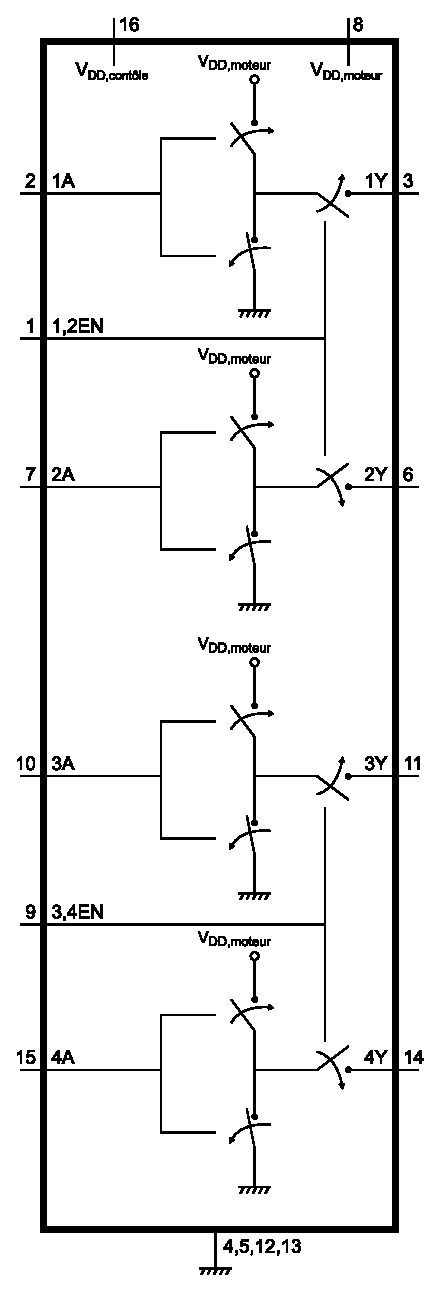
\includegraphics{L293.eps}
\caption{Schéma simplifié du L293D. Les numéros indiqués près des entrées/sorties correspondent aux numéros des broches de la puce.}
\label{L293}
\end{figure}


Vous pouvez maintenant réaliser sur une breadboard le petit circuit de contrôle illustré à la Figure~\ref{circuit}. Ce circuit utilise 2 demi-ponts H du L293. ATTENTION à ne pas oublier les diodes et à les connecter dans le bon sens. Comme expliqué précédemment, si ces diodes ne sont pas connectées correctement, le courant qui apparait lors de la décharge de l'énergie magnétique risquerait d'endommager le L293. N'hésitez pas à demander à l'un des membres du Club Elec de vérifier votre circuit si vous avez le moindre doute!\\

\begin{figure}[!t]
\centering
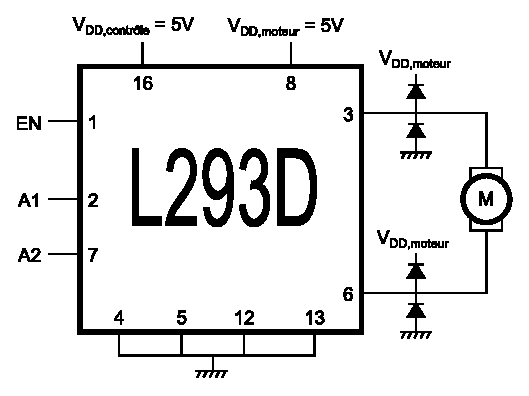
\includegraphics{circuit.eps}
\caption{Contrôle d'un moteur à l'aide du L293D. Les broches non indiquées sur le schéma peuvent être laissées flottantes ou connectées à la masse.}
\label{circuit}
\end{figure}

Essayez maintenant de connecter les signaux de contrôle (EN, A1, A2) à l'alimentation de 5V ou à la masse. Qu'observez-vous sur le moteur? Cela correspond-t-il bien à ce à quoi vous vous attendiez? Vérifiez avec le comportement attendu repris dans la Table~\ref{signal}.\\

\begin{table}[!t]
\caption{Signaux de contrôle pour le moteur DC}
\begin{center}
\begin{tabular}{|l|l|l|l|}
\hline
\textbf{EN}& \textbf{A1} & \textbf{A2} &\textbf{Moteur}\\
\hline
5V & 0V & 5V & Tourne dans un sens\\
5V & 5V & 0V & Tourne dans l'autre sens\\
5V & 0V & 0V & Freine\\
5V & 5V & 5V & Freine\\
0V & X & X & Libre\\
\hline
\end{tabular}
\label{signal}
\end{center}
\end{table}

S'il vous reste du temps, connectez l'entrée EN à un générateur de signal et générez un signal rectangulaire entre 0 et 5V. Que se passe-t-il lorsque vous faites varier le duty-cycle (rapport du temps à 5V et à 0V) de ce signal.


\section*{Contrôle du mouvement d'un robot}
Vous avez appris dans ce hands-on à contrôler des moteurs DC à partir de signaux de contrôle digitaux. Dans votre circuit, les valeurs de ces signaux de contrôle étaient fixées manuellement. Pour la suite de ce projet, vous recevrez, entre autres, un microcontrôleur de type Arduino qui permet d'envoyer des signaux de contrôle 5V, ainsi que 2 moteurs DC, un L293D et une pile 9V. Imaginez dès à présent la stratégie la plus efficace pour contrôler les mouvements de votre robot à partir de ce matériel. Voici quelques questions pour vous aiguiller:
\begin{itemize}
\item Quels sont les signaux à envoyer au L293D pour avancer? Et pour reculer?
\item Comment contrôler chacun des moteurs pour tourner?
\item Comment faire pour régler la vitesse du robot? 
\end{itemize}

\end{document}